\section{Methodology (1 page)}
\label{sec:methods}
In this section we will talk through the setup and methods that enabled us to track the changes in browser API usage, link pages that derive from the same kit, and evaluate our approach. 
The phishing pages themselves are taken from a variety of phishing feeds (OpenPhish\todocite{APWG}), PhishTank\todocite{APWG}), URLScan\todocite{APWG}), SMS Gateways from \todocite{us}, and APWG\todocite{APWG}) based on the availability of the feed, and the level access we had at the time. A breakdown of the timeline is given in Appendix-A. Each URL is then sent to an automated chromium crawler with the VisibleV8 patches applied to it\todocite{VV8}, and KitPhish, a URL fuzzing utility that helps identify left-behind phishing kits. The URLs are pulled from all feeds every 2 hours and only submitted for a crawl if the URL was not crawled within the last 1 week. The feed themselves either provide, or were filtered to URLs that have appeared on their blocklist only in the last 24 hours. 
\subsection{Data Gathering}

\subsubsection{VisibleV8 crawling}

The VisibleV8 crawler visits the pages for 45 seconds, gathering execution traces of browser APIs. 



\begin{figure}[t]
    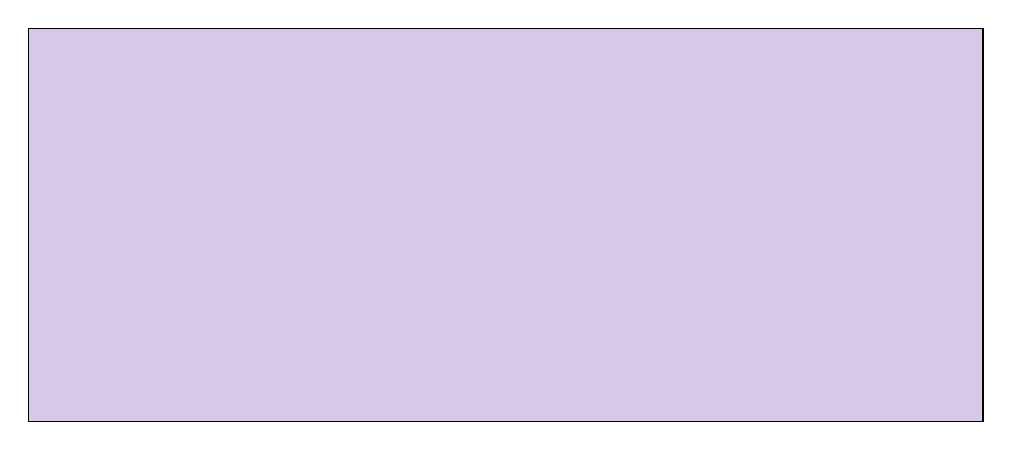
\begin{tikzpicture}
      \node[draw, fill=RoyalPurple!20, minimum width=\columnwidth, minimum height=5cm] {};
    \end{tikzpicture}
    \caption{Crawling infrastructure}
    \label{fig:infra}
    \Description["TODO: "]{"TODO"}
  \end{figure}
\subsection{Data enrichment}


We use the VisibleV8\todocite{VV8} patches to monitor the browser API calls and property accesses. We use the Chrome IDL data to filter out the browser API calls from the noise.

When we need further aggregation of the type of APIs we see, we use the MDN categories\todocite{MDN} to classify the APIs. We obtain these categories by processing the markdown files in the MDN repository.

To cut through the noise of cloaked pages and include third-party scripts like Google Analytics, which prior work shows and we confirm is used by phishing pages, we isolate API sets executed by first-party scripts (from now on called first-party API sets). To do this, we establish the root domain as the domain submitted to the feeds and the origin as the domain from which the script is loaded. We consider a script first-party only if loaded from the domain we acquired from our feeds (root domain). 

Since we limit our analysis to pages that execute javascript from the exact origin as the page submitted to the phishing feeds (submission origin), we effectively narrow our analysis to pages that do not engage in server-side cloaking by redirecting to a benign page or return an empty page. We discuss what we identify regarding javascript-based cloaking in \todocite{Section-Results}.

To establish which APIs are related to client-side cloaking as discussed by Zhang \etal{}\todocite{crawlphish}, we manually create a list of APIs that fall under the categories described in the paper. As well as query only the APIs that were listed in the paper.
\DraftToDo{Explain the difference\ldots{} Basically, there are more APIs if you consider Interaction as any click-related stuff and Fingerprint as ALL known FP APIs}

\begin{table}[t]
    
    \caption{Manual criteria to identify cloaking behavior established by Zhang \etal{}}
    \resizebox{\columnwidth}{!}{%\centering
    \begin{tabular}{cl}
        \textbf{Cloaking Category} & \multicolumn{1}{c}{\textbf{Required API calls}}                                                                                  \\ \hline
        User Interaction           & \begin{tabular}[c]{@{}l@{}}Any permission requesting API call\\ FilePicker API calls \\ HTMLElement event listeners\end{tabular} \\ \hline
        Fingerprinting             & \begin{tabular}[c]{@{}l@{}}HTMLDocument.cookie \\ HTMLDocument.referrer\\ Navigator.userAgent\end{tabular}                               \\ \hline
        Bot Behavior               & \begin{tabular}[c]{@{}l@{}}Crypto.getRandomBytes\footnote{Since Math.random is a javascript builtin function, VisibleV8 does not have visibility into it's execution}\\ Window.setTimeout + Performance.now\end{tabular}                          
        \end{tabular}
    }
\label{tab:behaviorcategories}
\end{table}
\subsection{Identifying trends }
For anomaly detection, we use rapture\todocite{ruptures} to detect changepoints in the time series of API calls. We use the L1 cost function with a linearly penalized segmentation algorithm to find segments based on the mean deviation.
To filter out noise in trends from the miss-balance of pages we get from different feeds, we ignore any API trends that strongly correlate with the number of pages we get from all feeds.
To clear up the results from rapture, we look at the change in the mean between segments. Any chance being less than XXXX, we ignore and merge with the prior segment. 
VisibleV8 will de-duplicate the same script loaded by multiple pages via the sha3 hash of the script. To establish if scripts have non-deterministic behavior, we pull the set of APIs that are executed by the script and compare the set of APIs executed by the same script on different pages. We use the Jaccard index to establish the similarity between the sets of APIs.

In \ref{sec:results}, we discuss APIs related to cloaking, obfuscation, and network IO. We hand-crafted these API lists by pulling from existing literature and adding any new APIs from the Mozila Developer's network. A complete list of the APIs can be found in the appendix. 

\subsection{Identifying kits}

The core hypothesis of this work is that similarity in browser API execution means that the pages originate from the same phishing kit. To establish this similarity, we use the Jaccard index on the set of APIs that first-party scripts execute. 
\DraftToDo{Well\ldots{} what about the whole merging clusters bit?}
We use HDBScan, with a minimum cluster size of 10, to cluster the pages based on the Jaccard index. We then use the ground truth labels from KitPhisher to evaluate the clustering. When ground truth is available, we use Fowlkes-Mallows Index (geometric mean between precision and recall)\todocite{Normalised Clustering Accuracy: An Asymmetric External Cluster Validity Measure}, and V-measure to evaluate the clustering.

V-measure is a harmonic mean between completeness (all members in a cluster are from the right class) and homogeneity (all members in a cluster are from the same class). V-measure allows tuning a ratio $\beta$ that prioritizes the score towards one vs the other. More importantly, looking at completeness and homogeneity scores lets you see how your clustering approach is getting things wrong.\todocite{V-Measure}
We use sklearn's measure module to calculate all cluster evaluation metrics.\todocite{sklearn}.

We use the silhouette score to evaluate the clustering when we do not have ground truth.
\DraftToDo{Go into detail why and mention that while SC is bias against DBSCAN/HDBSCAN, we still get good enough results where we are fine.}
\DraftToDo{Davies-Bouldin Index?}